
\documentclass[12pt]{article}
%	options include 12pt or 11pt or 10pt
%	classes include article, report, book, letter, thesis

\usepackage[margin=0.5in]{geometry}

\setlength{\parindent}{0pt}

\usepackage{hyperref}
\usepackage{graphicx}

%for writing of code in blocks like
%\begin{lstlisting}
%   .......
%\end{lstlisting}
\usepackage{listings}
\usepackage{color}
\usepackage{enumitem}

\definecolor{dkgreen}{rgb}{0,0.6,0}
\definecolor{gray}{rgb}{0.5,0.5,0.5}
\definecolor{mauve}{rgb}{0.58,0,0.82}

\lstset{frame=tb,
  language=C++,
  aboveskip=3mm,
  belowskip=3mm,
  showstringspaces=false,
  columns=flexible,
  basicstyle={\small\ttfamily},
  numbers=none,
  numberstyle=\tiny\color{gray},
  keywordstyle=\color{blue},
  commentstyle=\color{dkgreen},
  stringstyle=\color{mauve},
  breaklines=true,
  breakatwhitespace=true,
  tabsize=3
}
%%%%%%%%%%%%%%%%%%%%%%

\title{Life of a Particle : Assignment 2}
\author{Sam Meehan}
\date{Due Date : 13 January 2017}

\begin{document}
\maketitle

\textbf{How to Submit}
\newline
This assignment should be submitted by replying to the email sent out by the tutors - \textbf{Use the online form!} - with the link to your GitHub repository.  Contained within this repository should be a \href{https://github.com/adam-p/markdown-here/wiki/Markdown-Cheatsheet}{markdown README.md} file which provides a guide to the contents of the repository, along with instructions of how to run the code, where necessary.  For the full assignment, also include a well-written summary in the form of a latex document with one section per question.
\newline
\newline
\textbf{You are to work with the partner assigned to you as a team.}
\newline
\newline
\textbf{Coding Like a \href{https://www.urbandictionary.com/define.php?term=hipster}{Hipster} - (Just Directions)} 
\newline
You don't need to do any work here, these are just directions.  
\newline
\newline
For many common tasks, there are built in functions already existing in python, or which can be imported from the \small{\ttfamily{math}} or \small{\ttfamily{numpy}} modules.  In particular, the ones you may have used before are \small{\ttfamily{min(LIST)}}, \small{\ttfamily{max(LIST)}}, \small{\ttfamily{sum(LIST)}}, \small{\ttfamily{len(LIST)}}.  However, these are not necessary for ``good'' programmers.  Nearly all programs can be written using the following small set of operations 
\begin{itemize}[noitemsep]
\item $+$ (add)
\item $*$ (multiply
\item $/$ (divide)
\item $=$ (assignment)
\item $==$ (equals comparison)
\item $<$ (less than comparison)
\item $>$ (greater than comparison)
\end{itemize}
In addition to these operators, it is taken for granted in programming that you can use the following features as well
\begin{itemize}[noitemsep]
\item variables and lists - for storing the initial dataset
\item for loops
\item if statements
\item print statements - for viewing your code
\end{itemize}
In this quiz, these are the only things that may appear.   If you determine that you absolutely need some other function or operator, then include a comment clearly describing why this is the case.
\newline
\newline
Finally, you are not allowed to ``hard code'' in your program, meaning that there cannot be code that you must manually change each time you run it.  An example of this is the length of a list.  If I have a list [1,4,2,5,3,6], and you want to use the number of items in the list in your code, then the number ``6'' may not appear in your code.  
\newline
\newline
\newpage
\textbf{Standard Deviation Like a Hipster}
\newline
For this question, follow the directions to code like a ``hipster''.  Note that you can use the ROOT package to make histograms or graphs if you like.
\newline
\newline
Given a set of numbers $Q$ (example $Q=$[2,3,4,2]), write a program which calculates the standard deviation of this set.  For the purposes here, the definition of the standard deviation of a set of numbers is
\begin{displaymath}
\sigma(Q)=\sqrt{\frac{\displaystyle\sum_{i=0}^{N-1} (x_{i}-x_{avg})^2}{N}} 
\end{displaymath}
\begin{displaymath}
x_{avg}=\frac{\displaystyle\sum_{i=0}^{N-1} x_{i}}{N}
\end{displaymath}
\begin{displaymath}
N=N(Q)
\end{displaymath}
\newline
\textbf{NOTE!!!!}
\newline
For the following three ``hipster'' problems, choose one out of three to do.  That is, from the problems (Sorting, Dataset Correlation, Numerical Integration) choose to do only one for credit.  If you do one or both of the other two problem, they will count as \textit{BONUS}.
\newline
\newline
\textbf{[1] Sorting Like a Hipster}
\newline
For this question, follow the directions to code like a ``hipster''.  
\newline
\newline
Given this set of data (you can copy and paste it into an array if you like)
\newline
\newline
[71, 51, 32, 62, 84, 109, 43, 92, 72, 41, 102, 80, 72, 69, 46, 94, 52, 95, 90, 72, 63, 70, 34, 80, 78, 34, 31, 37, 26, 41, 42, 107, 33, 108, 108, 75, 66, 23, 90, 53, 24, 70, 26, 41, 93, 24, 71, 39, 48, 66, 97, 107, 77, 71, 67, 39, 38, 107, 96, 92, 84, 46, 60, 95, 87, 90, 92, 63, 78, 78, 84, 107, 70, 108, 32, 36, 93, 108, 49, 72, 56, 43, 30, 56, 51, 97, 45, 92, 40, 43, 49, 83, 98, 28, 99, 97, 102, 89, 58, 87]
\newline
\newline
write a program in python which sorts the data into an ascending array.  By this, I mean that the $0^{th}$ element in the list is the smallest, and the last element in the list is the largest.  If there is more than one element which has the same value, then the order of these two elements does not matter.  
\newline
\newline
\textbf{[2] Dataset Correlation Like a Hipster}
\newline
For this question, follow the directions to code like a ``hipster''.  
\newline
\newline
You are given a set of data in the format of $(x,y)$ pairs as can be found on the course website - \href{https://sites.google.com/a/aims.edu.gh/the-life-of-a-particle}{Course Website} - for assignment 2.  This data is formatted as
\begin{displaymath}
X=(x_0, x_1, x_2, ..., x_N) \textrm{  and  } Y=(y_0, y_1, y_2, ..., y_N)
\end{displaymath}
Given this dataset, calculate the ``linear correlation coefficient'' for this set of data as
\begin{displaymath}
\rho=\frac{V_{xy}}{\sigma_{x}\sigma_{y}} \textrm{  ,  } V_{xy}=E[xy]-\mu_{x}\mu_{y}
\end{displaymath}
where $E[xy]$ is the expectation value of the dataset $XY=(x_{0}y_{0}, x_{1}y_{1}, x_{2}y_{2}, ..., x_{N}y_{N})$ and $\mu$ and $\sigma$ are the standard deviation of the respective dataset.  I would recommend making a 2D histogram of this data in addition to doing some Googling about how to calculate the linear correlation coefficient as well.

\newpage
\textbf{[3] Numerical Integration Like a Hipster} 
\newline
For this question, follow the directions to code like a ``hipster''.  Note that you can use the ROOT package to make histograms or graphs if you like.
\newline
\newline
One of the most powerful tools in math is the integral.  In particular, this is powerful because it can be used to compute the area under a curve, a concept which can be generalized to refer to volumes or more complicated quantities, like the amount of work performed on a particle by an electric field as the particle moves through a trajectory.  One typically learns to compute (definite) integrals as
\begin{displaymath}
I_{y(x)}(a,b)=\displaystyle\int_{a}^{b} x^n dx = \frac{x^{n-1}}{n-1}|_{x=a}^{x=b} =  \frac{1}{n-1}(b^{n-1}-a^{n-1})
\end{displaymath}
and this can be used to compute more complicated integrals like
\begin{displaymath}
I_{y(x)}(a,b)=\displaystyle\int_{a}^{b} y(x) dx 
\end{displaymath}
However, there is another method to compute the definite integral $I$ computationally called a \textit{Riemann Sum}.  Graphically, it proceeds as shown in Figure~\ref{fig:riemann}.  The integral is \textbf{approximated} by a sum of the are of the rectangles of some width ($\Delta x$) with a height equal to $y(x_{eval})$ where $y(x_{eval})$ can be evaluated at the (i) left, (ii) right, or (iii) middle of the rectangle.  In this case, the value of the integral is
\begin{displaymath}
I_{y(x)}(a,b)\sim \displaystyle\sum_{i=0}^{N-1} y(x_{i})\times(x_{i+1}-x_{I})=\displaystyle\sum_{i=0}^{N-1} y(x_{i})\times\Delta x
\end{displaymath}
Now, typically (but not necessarily) the value of $\Delta x$ is fixed and taken to be $\Delta x=\frac{b-a}{N}$.  Now, if you remember integral calculus, then you will remember that
\begin{displaymath}
 \displaystyle\lim_{N\to\infty} \displaystyle\sum_{i=0}^{N-1} y(x_{i})\times\Delta x = \displaystyle\int_{a}^{b} y(x) dx 
\end{displaymath}
Therefore, we can calculate the integral by writing a piece of code that performs this definite sum!  So, the task is to write a piece of python code which performs the integral of $y(x)=3x^3-4x^2+3.2198x$ from $a=1$ to $b=9$.  Perform this calculation analytically and then perform it numerically using your code for $N=$[10,50,100,200].  How close does this approximation approach to the analytic result.
\begin{figure}[h!]
  \center
  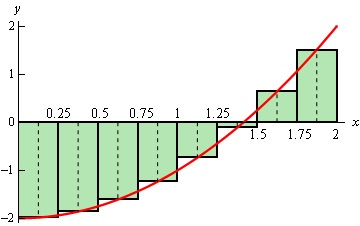
\includegraphics[width=0.5\linewidth]{riemann}
  \caption{An illustration of the Riemann sum used to approximate the integral of the function $y(x)$ (the red curve) from $x=$0 to $x=$2.  In this case, the step size $\Delta x$ is taken to be 0.25 and the function $y(x)$ is evaluated at the center point of each interval.}
  \label{fig:riemann}
\end{figure}

\newpage
\textbf{Fitting a Line} 
\newline
For this question, follow the directions to code like a ``hipster''.  Note that you can use the ROOT package to make histograms or graphs if you like.
\newline
\newline
One procedure that is used regularly in computational modelling is that of ``fitting''.  This itself is a very broad topic and here we will implement one of the more basic procedures called the \href{https://en.wikipedia.org/wiki/Least_squares}{``minimization of least squares''}.  To make this concrete, let's pretend that you have measurements of a particles position at equal time intervals and obtain the following measurements :
\begin{center}
\begin{tabular}{ c|c } 
 x [m] & y [m] \\ \hline
 1.0 & 0.5 \\ 
 2.2 & 1.1 \\ 
 3.0 & 1.3 \\
 3.9 & 2.1 \\
 4.8 & 2.6 \\
\end{tabular}
\end{center}
Now, you have a good reason to believe that this particle is moving on a straight line path, but your eyesight is not good and if you plot these points on a scatter plot, they don't seem to be perfectly along a straight line.  Nonetheless, you would like to determine the functional form of the path followed by the particle, which you know to be $y=f(x;m,b)=m\times x+b$.  To do this, you can use the ``minimization of least squares'' as follows :
\begin{itemize}
\item Choose values for the parameters $(m,b)$
\item Calculate the value of the fit error which equals $S=\displaystyle\sum_{points} (f(x_{i})-y_{i})^{2}$ as represented graphically in Figure~\ref{fig:fit}.
\item Make a list which matches a single choice of $(m,b)$ to a value of $S$ and fill it with many $(m,b,S)$ choices
\item Find the entry in this list of $(m,b,S)$ which has the smallest value of $S$.  The corresponding $(m,b)$ values are what we call the ``best fit'' values of the parameters of our models.
\end{itemize}
Use this procedure to determine the best fit values of the line which describes the data you observed and create a plot of the data points and your best fit line.

\begin{figure}[h!]
  \center
  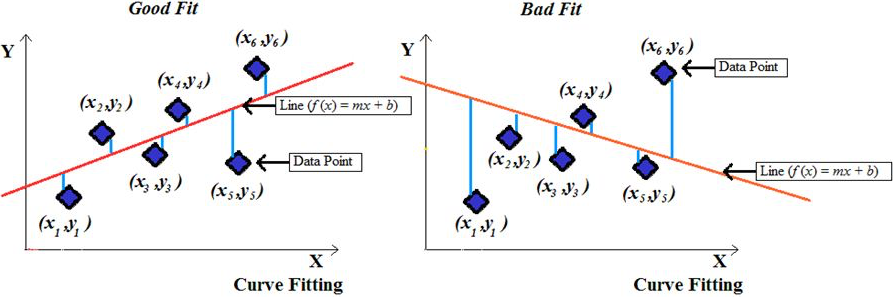
\includegraphics[width=0.7\linewidth]{fit}
  \caption{An illustration of the procedure to minimize the fit error and thereby determine the model parameters $m$ and $b$ that best describe our data.}
  \label{fig:fit}
\end{figure}

\newpage
\textbf{The Logistic Map} 
\newline
This is the completion of what we started in class.  You are to work through the exercise of creating code that reproduces the results in this paper - \href{http://dtic.mil/dtic/tr/fulltext/u2/a282268.pdf}{the logistic map paper}.  In short, you should be recreating the histograms in this paper that demonstrate the behavior of the sequence of $X$ values produced directly from the logistic map, and the sequence of $Y$ values that are produced from the transformed logistic map.  Use both one-dimensional and two-dimensional histograms to inspect the bias of both $X$ and $Y$. 
\newline
\newline
\textbf{Gaussian Random Numbers} 
\newline
For this question, you may import the \href{https://docs.python.org/2/library/random.html}{python random library}.  However, you may only use the \href{https://docs.python.org/2/library/random.html#random.random}{random.random()} function call which generates a uniformly distributed random number between [0,1.0).
\newline
\newline
Starting from a set of uniformly distributed random numbers from [0,1.0) (Don't be a hipster, use python for this!) generate a set of 10000 random numbers according to a \href{https://en.wikipedia.org/wiki/Gaussian_function}{Gaussian distribution} of mean $\mu=2.0$ and width $\sigma=1.4$.  As a reminder, the Gaussian distribution is also called the ``normal distribution'' and has the following functional form :
\begin{displaymath}
 Gauss(x;\mu,\sigma)=\frac{1}{\sigma\sqrt{2\pi}}Exponential[-\frac{1}{2} (\frac{x-\mu}{\sigma})^{2}]
\end{displaymath}
where $Exponential[a]=e^{a}$.  Use the accept-reject method and limit the range of your generation to $x\in [-10,10]$.







\end{document}